% -*-coding: utf-8 -*-

\defaultfont

\BiChapter{水下绳驱机械臂轨迹规划与仿真}{To Template Maintainers}

\BiSection{引言}{Simple Introduction about This Template}



常用的机械臂轨迹规划方法可分为两类：一类是在关节空间中进行规划，用户对选定的插值点上的位姿、
速度、加速度给出显式约束（如连续性、光滑性），规划器采用多项式等函数对节点进行插值。该方法
计算简单、关节运动平滑，但由于未对末端笛卡尔路径施加直接约束，用户难以预知末端的实际空间轨
迹，存在与障碍物碰撞的风险。另一类是在笛卡尔空间中进行规划，用户直接给出末端运动路径的解析
表达式（如直线、圆弧），规划器在关节空间或笛卡尔空间中逼近预定路径。该方法能直观控制末端轨
迹，便于避障，但需实时求解逆运动学，计算负担较重。

本文所研究的水下绳驱机械臂具有三自由度、关节耦合性强、驱动后置等特点，前文已建立其改进 D-H 
运动学模型及驱动空间到关节空间的映射关系。为实现机械臂在水下复杂环境中的平稳、精确作业，本
章将综合关节空间与笛卡尔空间规划的优势，分别开展基于多项式插值的关节空间轨迹规划与基于直线
/圆弧插补的笛卡尔空间轨迹规划，并利用 MATLAB 进行数值仿真，对比分析两种方法在末端轨迹精度、
关节速度/加速度连续性及计算效率等方面的表现，为后续控制系统设计提供理论依据。

\BiSection{关节空间轨迹规划}{Maintaining Tools Introduction}

关节空间轨迹规划的目标是在给定起始位姿和目标位姿的情况下，通过插值算法生成一系列连续的关节角度、角速度及角加速度序列，从而驱动机械臂完成预定任务。
在水下环境中，为了减小机械臂运动对水体的扰动并避免激起瞬时高载荷，轨迹规划需满足：
连续性和平稳性，及关节位置、速度及加速度必须连续，同时为了保证电机不被损坏 需满足关节转角范围、最大角速度及最大角加速度约束。
\BiSubsection{多项式插值规划算法}{Subsubsection}

传统的低阶多项式（如三次多项式）虽能保证位置与速度连续，但在起步与停止时刻会产生加加速度的无穷大突变，进而引起机械结构振动并对水体产生冲击扰动。为了彻底消除这一缺陷，本研究采用五次多项式来描述关节角度随时间变化的规律。

设关节在 $t=0$ 时刻的初始状态为：位置 $q_0$、速度 $v_0$、加速度 $a_0$；在作业时间 $t=T$ 时刻的末端状态为：位置 $q_f$、速度 $v_f$、加速度 $a_f$。据此可构建关于时间 $t$ 的五次多项式位置函数及其一阶导数（速度方程）和二阶导数（加速度方程）：

\begin{equation}
    q(t) = c_0 + c_1 t + c_2 t^2 + c_3 t^3 + c_4 t^4 + c_5 t^5
\end{equation}
\begin{equation}
    \dot{q}(t) = c_1 + 2c_2 t + 3c_3 t^2 + 4c_4 t^3 + 5c_5 t^4
\end{equation}
\begin{equation}
    \ddot{q}(t) = 2c_2 + 6c_3 t + 12c_4 t^2 + 20c_5 t^3
\end{equation}

将轨迹规划的始末边界条件代入上述方程，可得到如下 $6 \times 6$ 的约束方程组：

\begin{equation}
    \begin{cases}
        q(0) = c_0 = q_0 \\
        \dot{q}(0) = c_1 = v_0 \\
        \ddot{q}(0) = 2c_2 = a_0 \\
        q(T) = c_0 + c_1 T + c_2 T^2 + c_3 T^3 + c_4 T^4 + c_5 T^5 = q_f \\
        \dot{q}(T) = c_1 + 2c_2 T + 3c_3 T^2 + 4c_4 T^3 + 5c_5 T^4 = v_f \\
        \ddot{q}(T) = 2c_2 + 6c_3 T + 12c_4 T^2 + 20c_5 T^3 = a_f
    \end{cases}
\end{equation}

为了便于在计算系统中进行离散化求解，将其转换为矩阵表达形式：

\begin{equation}
    \begin{bmatrix}
        1 & 0 & 0 & 0 & 0 & 0 \\
        0 & 1 & 0 & 0 & 0 & 0 \\
        0 & 0 & 2 & 0 & 0 & 0 \\
        1 & T & T^2 & T^3 & T^4 & T^5 \\
        0 & 1 & 2T & 3T^2 & 4T^3 & 5T^4 \\
        0 & 0 & 2 & 6T & 12T^2 & 20T^3
    \end{bmatrix}
    \begin{bmatrix}
        c_0 \\ c_1 \\ c_2 \\ c_3 \\ c_4 \\ c_5
    \end{bmatrix}
    =
    \begin{bmatrix}
        q_0 \\ v_0 \\ a_0 \\ q_f \\ v_f \\ a_f
    \end{bmatrix}
\end{equation}

通过矩阵求逆及代数消元运算，可解析得出该多项式轨迹方程的全部待定系数：

\begin{equation}
    \begin{cases}
        c_0 = q_0 \\
        c_1 = v_0 \\
        c_2 = \frac{a_0}{2} \\
        c_3 = \frac{20(q_f - q_0) - (8v_f + 12v_0)T - (3a_0 - a_f)T^2}{2T^3} \\
        c_4 = \frac{-30(q_f - q_0) + (14v_f + 16v_0)T + (3a_0 - 2a_f)T^2}{2T^4} \\
        c_5 = \frac{12(q_f - q_0) - 6(v_f + v_0)T - (a_0 - a_f)T^2}{2T^5}
    \end{cases}
\end{equation}

将上述系数代回原多项式，即可生成机械臂在给定时间 $T$ 内平滑且完全满足运动学约束的理想轨迹。

\BiSubsection{梯形速度规划算法}{Subsubsection}

在水下环境执行摄像扫描、结构物检测或目标抓取等任务时，常要求机械臂末端在特定工作空间内保持平稳的匀速运动。此时，采用具有抛物线过渡的线性插值，即梯形速度规划算法具有更高的工程实用性。

梯形速度规划通过分段函数将整个运动周期划分为三个核心区间：匀加速段、匀速作业段与匀减速段。设关节的起始位置为 $q_0$，目标位置为 $q_f$，系统允许的最大运行角速度为 $v_{max}$，最大允许加速度为 $a_{max}$。

若给定的目标路径长度足以支撑系统加速至最高速度，即满足阈值条件 $|q_f - q_0| > \frac{v_{max}^2}{a_{max}}$ 时，系统的加速时间 $t_a$ 及总运行时间 $T$ 定义为：

\begin{equation}
    t_a = \frac{v_{max}}{a_{max}}, \quad T = \frac{|q_f - q_0|}{v_{max}} + t_a
\end{equation}

在不失一般性的前提下，假设 $q_f > q_0$ 且系统的起止速度均为 $0$，该规划算法在时间轴上的分段运动学方程如下：

\textbf{（1）匀加速段 ($0 \le t \le t_a$)}

此阶段机械臂电机输出恒定大扭矩，以最大加速度 $a_{max}$ 启动，其运动方程为：
\begin{equation}
    \begin{cases}
        q(t) = q_0 + \frac{1}{2} a_{max} t^2 \\
        \dot{q}(t) = a_{max} t \\
        \ddot{q}(t) = a_{max}
    \end{cases}
\end{equation}

\textbf{（2）匀速作业段 ($t_a < t \le T - t_a$)}

达到设定巡航速度后，系统加速度降为 $0$，保持 $v_{max}$ 匀速运行以提升作业质量：
\begin{equation}
    \begin{cases}
        q(t) = q_0 + \frac{1}{2} a_{max} t_a^2 + v_{max} (t - t_a) \\
        \dot{q}(t) = v_{max} \\
        \ddot{q}(t) = 0
    \end{cases}
\end{equation}

\textbf{（3）匀减速段 ($T - t_a < t \le T$)}

临近目标点时，机械臂以反向最大加速度 $-a_{max}$ 平滑制动：
\begin{equation}
    \begin{cases}
        q(t) = q_f - \frac{1}{2} a_{max} (T - t)^2 \\
        \dot{q}(t) = v_{max} - a_{max}(t - (T - t_a)) \\
        \ddot{q}(t) = -a_{max}
    \end{cases}
\end{equation}

特别地，在算法设计时需要考虑退化情况。若规划的目标位移过短（即 $|q_f - q_0| \le \frac{v_{max}^2}{a_{max}}$），系统在达到最大设定速度前即需触发减速指令。此时梯形速度曲线退化为三角形速度曲线，算法必须自适应重新计算实际可达的峰值速度 $v'_{max} = \sqrt{|q_f - q_0| a_{max}}$，并将匀速段运行时间置为零以防止位置超调。

\BiSubsection{仿真与结果分析}{Subsubsection}


\section{仿真实验与结果分析}

为了验证本文所提出的五次多项式插值算法与梯形速度规划算法在水下绳驱机械臂关节空间轨迹规划中的
有效性，本章利用 MATLAB 仿真平台进行数值仿真对比。通过分析关节的位置、速度、加速度及加加速度
曲线，评估算法在平滑性、作业效率以及对水下环境影响等方面的表现。

\subsection{仿真环境与参数设置}

实验设定机械臂某关节从起始角度 $q_0 = 0^\circ$ 运动至目标角度 $q_f = 90^\circ$。为了确保仿真的真实性，结合水下电机的物理性能及流体阻力约束，设定了最大速度与加速度限制。具体仿真参数如表 \ref{tab:params} 所示。

\begin{table}[htbp]
\centering
\caption{关节空间轨迹规划仿真参数}
\label{tab:params}
\begin{tabular}{lcc}
\hline
\textbf{参数名称} & \textbf{符号} & \textbf{设定值} \\ \hline
起始位置 (Start Position) & $q_0$ & $0^\circ$ \\
目标位置 (Final Position) & $q_f$ & $90^\circ$ \\
最大允许速度 (Max Velocity) & $v_{max}$ & $20^\circ/s$ \\
最大允许加速度 (Max Acceleration) & $a_{max}$ & $10^\circ/s^2$ \\
仿真步长 (Time Step) & $\Delta t$ & $0.01s$ \\
\hline
\end{tabular}
\end{table}

\subsection{仿真结果分析}

基于上述参数，分别运行梯形速度规划与五次多项式插值算法，得到对比曲线并分析如下：
\begin{figure}[H] % htbp代表图片插入位置的设置
    \centering %图片居中
    %添加图片；[]中为可选参数，可以设置图片的宽高；{}中为图片的相对位置
    
\includegraphics[width = \textwidth]{关节插值}
    \caption{对比曲线} % 图片标题
    \label{pic41} % 图片标签
    \end{figure}
\begin{enumerate}
    \item \textbf{位置曲线分析}：
    如图\ref{pic41}所示，两种算法均能准确地在预定时间内引导关节从起始位移到达目标位移。梯形速度规划在中间段表现出明显的线性增长（匀速段），而五次多项式轨迹则呈现出更为圆滑的“S”型曲线。
    
    \item \textbf{速度与加速度分析}：
    梯形速度规划在加速段和减速段保持恒定的加速度，这虽然缩短了运动时间，但其加速度曲线在 $t=t_a$ 等时刻存在明显的阶跃突变（见图 2）。相比之下，五次多项式算法的速度曲线呈平滑的钟形分布，加速度曲线连续且在始末状态均为 0，能够显著降低由于惯性力突变带来的冲击。
    
    \item \textbf{加加速度分析}：
    加加速度 曲线是评价系统平稳性的核心指标。梯形规划在速度转换点处的 加加速度 趋于无穷大，表现为脉冲形式。这对于绳驱系统而言，极易诱发绳索的弹性颤动，甚至导致绳索在瞬间松弛后又被剧烈张紧，严重影响使用寿命。五次多项式规划的 加加速度 曲线幅值有限且连续，展现了极佳的柔顺性。
\end{enumerate}


综上所述，实验结果表明：
\begin{itemize}
    \item \textbf{梯形速度规划}适用于对作业效率要求较高、且具有明确匀速作业需求的场景。
    \item \textbf{五次多项式插值}虽然在运动时间上略长，但其在加速度连续性及震动抑制方面具有压倒性优势。
\end{itemize}
综合考虑水下绳驱机械臂的柔性特性与流体环境干扰，本文后续研究将优先采用五次多项式规划作为底层控制的参考输入。



\BiSection{笛卡尔空间轨迹规划}{Subsubsection}

笛卡尔空间轨迹规划直接描述机械臂末端执行器在作业空间中的运动几何特征。对于水下绳驱机械臂而言，其作业任务（如焊缝跟踪、圆周扫描）通常定义在笛卡尔坐标系下。

本研究采用“路径离散化，关节空间连续规划”的策略：即首先根据几何约束生成笛卡尔空间的离散点集，通过逆运动学将位姿序列映射为关节角序列，最后在关节空间完成平滑化处理。

\BiSubsection{直线轨迹规划}{Subsubsection}

直线运动是机械臂末端在起始点 $\mathbf{P}_s$ 与目标点 $\mathbf{P}_e$ 之间沿最短路径移动的过程。

（1）参数化路径生成

如图\ref{pic42}，设起始位置向量为 $\mathbf{P}_s = [x_s, y_s, z_s]^T$，终点向量为 $\mathbf{P}_e = [x_e, y_e, z_e]^T$。定义路径参数 $s \in [0, 1]$，则空间直线的几何参数方程为：
\begin{equation}
    \mathbf{P}(s) = \mathbf{P}_s + s(\mathbf{P}_e - \mathbf{P}_s)
\end{equation}

\begin{figure}[H] % htbp代表图片插入位置的设置
    \centering %图片居中
    %添加图片；[]中为可选参数，可以设置图片的宽高；{}中为图片的相对位置
    
\includegraphics[width = 0.5\textwidth]{直线.jpg}
    \caption{直线轨迹} % 图片标题
    \label{pic42} % 图片标签
    \end{figure}
（2）路径离散化

给定采样周期 $\Delta t$ 和期望运行速度 $v_d$，总运动距离 $L = \|\mathbf{P}_e - \mathbf{P}_s\|$，总采样点数 $N$ 定义为：
\begin{equation}
    N = \lceil \frac{L}{v_d \cdot \Delta t} \rceil
\end{equation}
生成的离散点序列 $\mathcal{P}_{line} = \{ \mathbf{P}_0, \mathbf{P}_1, \dots, \mathbf{P}_N \}$ 中，任一点的坐标计算公式如下：
\begin{equation}
    \mathbf{P}_k = \mathbf{P}_s + \frac{k}{N}(\mathbf{P}_e - \mathbf{P}_s), \quad k = 0, 1, \dots, N
\end{equation}

\BiSubsection{圆弧轨迹规划}{Subsubsection}

圆弧规划采用“空间三点定圆”法，通过起点 $\mathbf{P}_0$、途径点 $\mathbf{P}_1$ 及终点 $\mathbf{P}_2$ 确定唯一的空间圆弧轨迹。

（1）空间几何模型建立

如图\ref{pic43},定义两向量 $\mathbf{v}_1 = \mathbf{P}_1 - \mathbf{P}_0$ 和 $\mathbf{v}_2 = \mathbf{P}_2 - \mathbf{P}_0$。通过向量叉乘获得圆弧平面单位法向量 $\mathbf{n}_w$：




\begin{equation}
    \mathbf{n}_w = \frac{\mathbf{v}_1 \times \mathbf{v}_2}{\|\mathbf{v}_1 \times \mathbf{v}_2\|}
\end{equation}

建立局部平面坐标系 $O_{local} - \{ \mathbf{u}, \mathbf{v} \}$，其中 $\mathbf{u} = \frac{\mathbf{v}_1} { \|\mathbf{v}_1\|}$，$\mathbf{v} = \mathbf{n}_w \times \mathbf{u}$。通过几何投影法，解得圆心在局部坐标系下的坐标 $(c_u, c_v)$ 及半径 $R$：
\begin{equation}
    c_u = \frac{\|\mathbf{v}_1\|}{2}, \quad c_v = \frac{\mathbf{v}_2 \cdot \mathbf{v}_2 - \mathbf{v}_2 \cdot \mathbf{v}_1}{2 \mathbf{v}_2 \cdot \mathbf{v}}
\end{equation}
进而得到世界坐标系下的空间圆心 $\mathbf{P}_c = \mathbf{P}_0 + c_u \mathbf{u} + c_v \mathbf{v}$。

\begin{figure}[H] % htbp代表图片插入位置的设置
    \centering %图片居中
    %添加图片；[]中为可选参数，可以设置图片的宽高；{}中为图片的相对位置
    
\includegraphics[width = 0.5\textwidth]{圆弧.jpg}
    \caption{圆弧轨迹} % 图片标题
    \label{pic43} % 图片标签
    \end{figure}

（2）路径离散化


定义圆心指向起点及终点的单位向量为 $\mathbf{r}_s = \frac{(\mathbf{P}_0 - \mathbf{P}_c)}{R}$ 和 $\mathbf{r}_e = \frac{(\mathbf{P}_2 - \mathbf{P}_c)}{R}$。总旋转角度 $\theta_{total}$ 为两向量夹角。
在第 $k$ 个采样时刻，圆弧路径点 $\mathbf{P}_k$ 为：
\begin{equation}
    \mathbf{P}_k = \mathbf{P}_c + R \left[ \cos(\frac{k}{M} \theta_{total}) \mathbf{r}_s + \sin(\frac{k}{M} \theta_{total}) (\mathbf{n}_w \times \mathbf{r}_s) \right]
\end{equation}
其中 $M$ 为根据切向速度约束计算的圆弧采样总点数。

\BiSubsection{笛卡尔空间至关节空间}{Simple Introduction about This
Template}
本研究的核心逻辑是将上述生成的笛卡尔点序列转化为关节空间的控制指令，流程如图~\ref{pic44} 所示。



\begin{figure}[H] % htbp代表图片插入位置的设置
    \centering %图片居中
    %添加图片；[]中为可选参数，可以设置图片的宽高；{}中为图片的相对位置
    
\includegraphics[width = \textwidth]{流程图.jpg}
    \caption{算法流程图} % 图片标题
    \label{pic44} % 图片标签
    \end{figure}




（1）逐点逆运动学映射

对于生成的点序列 $\mathcal{P} = \{ \mathbf{P}_0, \mathbf{P}_1, \dots, \mathbf{P}_n \}$，通过逆运动学函数 $IK(\cdot)$ 求解对应的关节角序列 $\mathcal{Q} = \{ \mathbf{q}_0, \mathbf{q}_1, \dots, \mathbf{q}_n \}$：
\begin{equation}
    \mathbf{q}_k = IK(\mathbf{P}_k, \mathbf{q}_{k-1}), \quad k \in [1, n]
\end{equation}
其中，引入前一时刻解 $\mathbf{q}_{k-1}$ 作为当前解算的参考，目的是在逆运动学存在多解的情况下，选择与前一位置距离最短的配置，确保关节运动的连续性，规避“跳解”风险。

（2）关节空间轨迹衔接与平滑

由于映射得到的 $\mathbf{q}_k$ 序列本质上是离散的关节角指令，直接驱动电机可能导致角速度
不连续。因此，在相邻两点 $\mathbf{q}_k$ 与 $\mathbf{q}_{k+1}$ 之间，采用前述的五次多项
式进行微段插值。该方法不仅保证了末端执行器严格沿预设路径（直线或圆弧）运动，还确保了各
关节在启动、运行及停止时刻的加速度连续。

\BiSection{轨迹规划仿真与结果分析}{Simple Introduction about This
Template}




为了验证本文所提出的笛卡尔空间离散插补算法及逆运动学映射策略的有效性，本章利用 MATLAB 
仿真平台，针对水下绳驱机械臂的两种典型作业工况——直线运动与空间圆弧运动进行了仿真实验。

\BiSubsection{仿真环境与参数设置}{Subsubsection}

仿真实验基于机械臂的改进 DH 参数模型进行。为了模拟实际控制系统的运行环境，设定系统采样
周期 $\Delta t = 0.05$s，末端期望最大运动速度 $v_{max} = 0.06$m/s。机械臂各关节的运动
范围约束如表 \ref{tab:joint_limits} 所示。

\begin{table}[htbp]
    \centering
    \caption{机械臂关节运动空间约束}
    \label{tab:joint_limits}
    \begin{tabular}{ccc}
        \hline
        关节序号 & 物理约束范围 & 运动学定义 \\ \hline
        Joint 1 & $[-90^\circ, 90^\circ]$ & 水平回转角度 \\
        Joint 2 & $[0^\circ, 90^\circ]$ & 升降大臂角度 \\
        Joint 3 & $[0^\circ, 180^\circ]$ & 俯仰小臂角度 \\ \hline
    \end{tabular}
\end{table}


\BiSubsection{直线轨迹规划仿真分析}{Subsubsection}
设定直线运动的起始点 $P_s = (0.6, -0.2, 0.3)$，终止点 $P_e = (0.6, 0.2, 0.5)$。

圆弧路径通过空间三点 $P_0(0.5, -0.2, 0.4)$、$P_1(0.6, 0, 0.5)$、$P_2(0.5, 0.2, 0.4)$。

\BiSubsection{运动特性分析}{Subsubsection}

如图 \ref{fig:total_figure45} 所示，机械臂末端在笛卡尔空间内严格遵循预设的路径。通过提
取运动过程中的位姿叠影图可以看出，机械臂各连杆在空间中的过渡平滑。有效地抑制了关节解在
多解空间中的跳变。
\begin{figure}[H]
    \centering
    % 第一张子图
    \begin{minipage}{0.45\textwidth}
        \centering
        \subfigure[直线路径]{\label{fig45:sub1}
            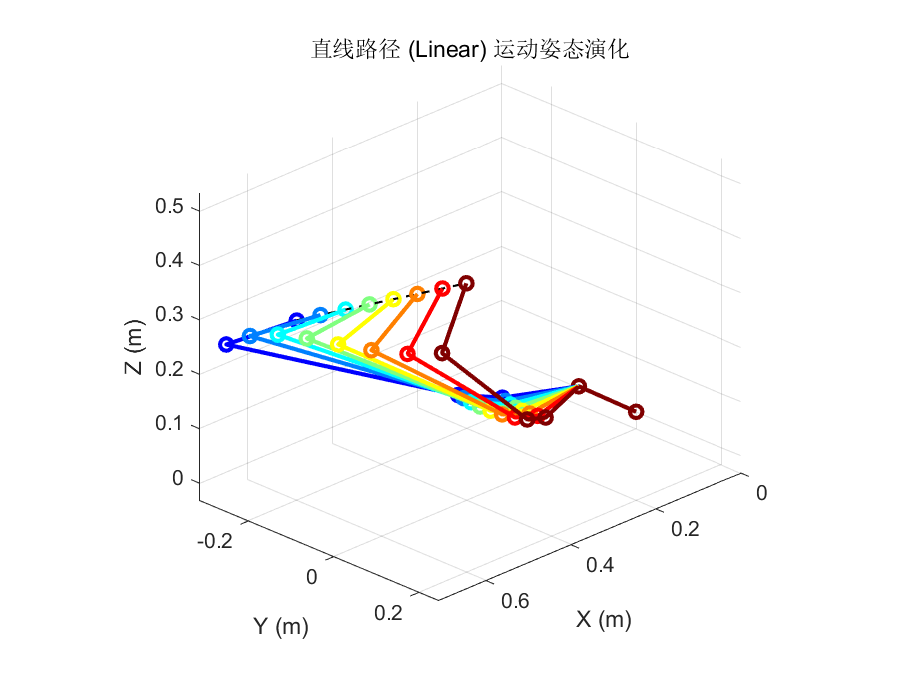
\includegraphics[width =\textwidth]{figures/直线演化.eps}
        }% 这里写第一张图的英文描述
    \end{minipage}
    % \hfill % 撑开左右间距
    % 第二张子图
    \begin{minipage}{0.45\textwidth}
        \centering
        \subfigure[圆弧路径]{\label{fig45:sub2}
            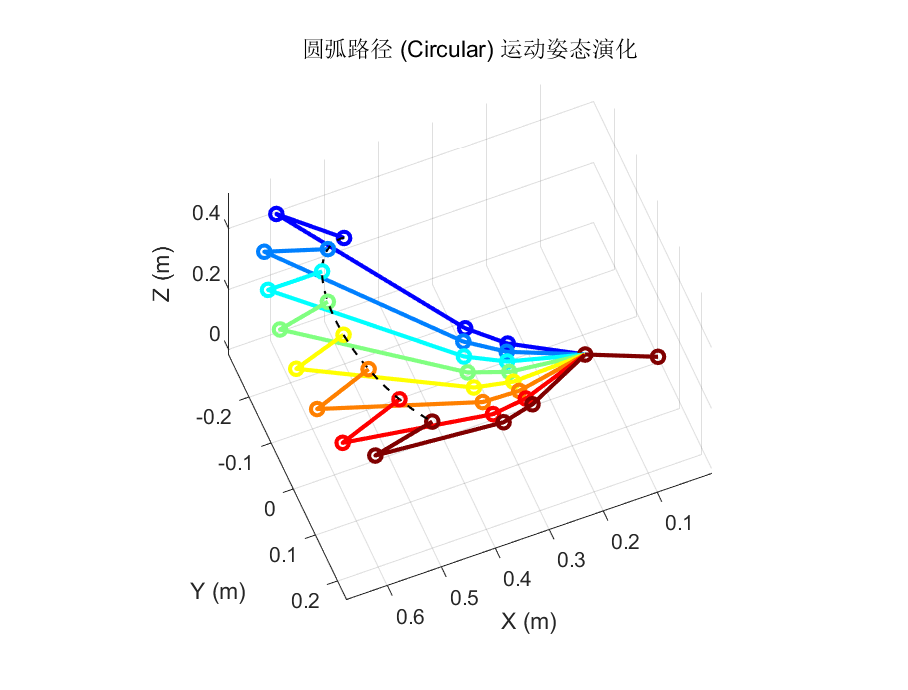
\includegraphics[width = \textwidth]{figures/圆弧演化.eps}
        } % 这里写第二张图的英文描述
             % 第一张子图
            \end{minipage}
    % 中英文总标题
    \caption{肘关节耦合原理}
    \label{fig:total_figure45}
  \end{figure}


\BiSubsection{关节空间响应}{Subsubsection}

从图 \ref{pic46} 的关节角度与速度曲线可以看出，各关节在运动起点与终点的速度均经过平滑
过渡，角速度曲线连续且无剧烈脉冲。这证明了本文采用的离散化插补策略能够为底层电机驱动
器提供高质量的输入信号，避免机械震动。


\begin{figure}[H]
    \centering
    % 第一张子图
    \begin{minipage}{0.45\textwidth}
        \centering
        \subfigure[直线路径]{\label{fig45:sub1}
            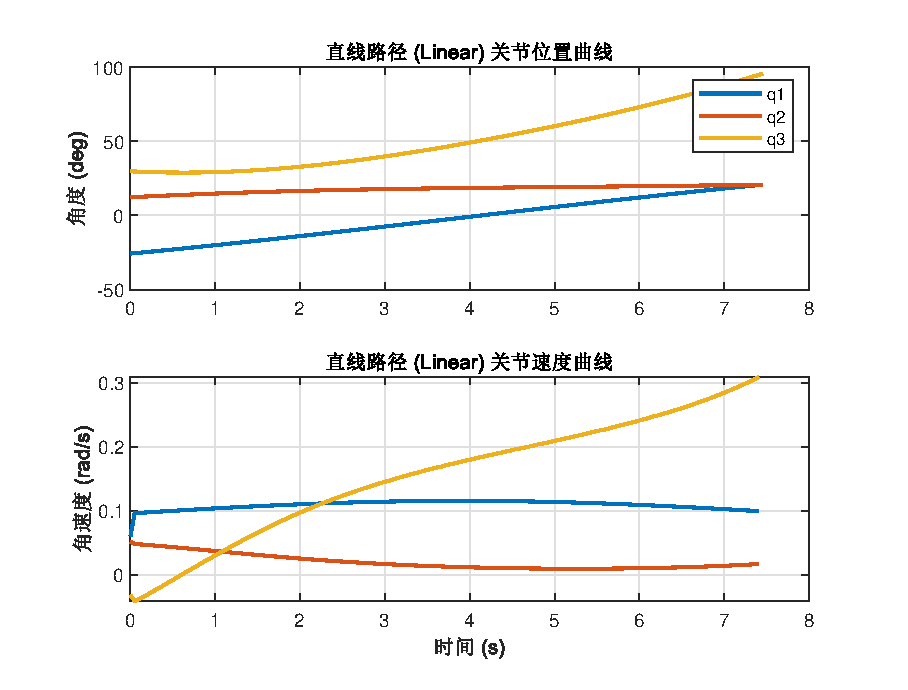
\includegraphics[width =\textwidth]{figures/直线关节.eps}
        }% 这里写第一张图的英文描述
    \end{minipage}
    % \hfill % 撑开左右间距
    % 第二张子图
    \begin{minipage}{0.45\textwidth}
        \centering
        \subfigure[圆弧路径]{\label{fig45:sub2}
            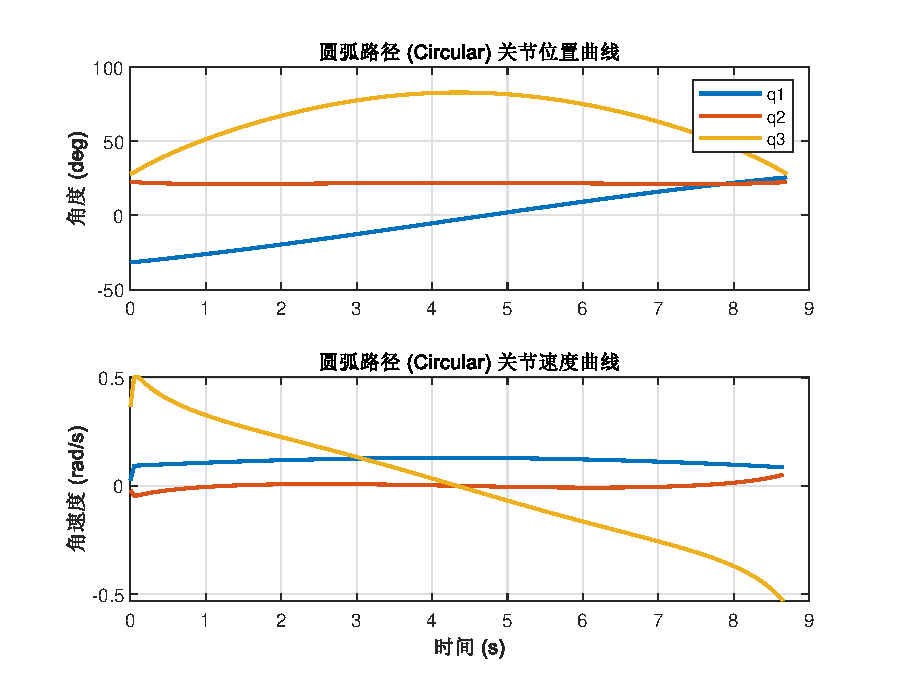
\includegraphics[width = \textwidth]{figures/圆弧关节.eps}
        } % 这里写第二张图的英文描述
             % 第一张子图
            \end{minipage}
    % 中英文总标题
    \caption{关节角度与速度曲线}
    \label{pic46}
  \end{figure}
\BiSubsection{跟踪精度评价}{Subsubsection}

针对空间轨迹，本文算法表现出了极高的跟踪精度。如图 \ref{pic47} 所示，末端执行器在整
个运动周期内的欧氏距离误差保持在 $10^{-2}$mm 量级。平均误差为 $0.042$mm。

\begin{figure}[H]
    \centering
    % 第一张子图
    \begin{minipage}{0.45\textwidth}
        \centering
        \subfigure[直线路径]{\label{fig46:sub1}
            \includegraphics[width =\textwidth]{figures/直线精度.eps}
        }% 这里写第一张图的英文描述
    \end{minipage}
    % \hfill % 撑开左右间距
    % 第二张子图
    \begin{minipage}{0.45\textwidth}
        \centering
        \subfigure[圆弧路径]{\label{fig46:sub2}
            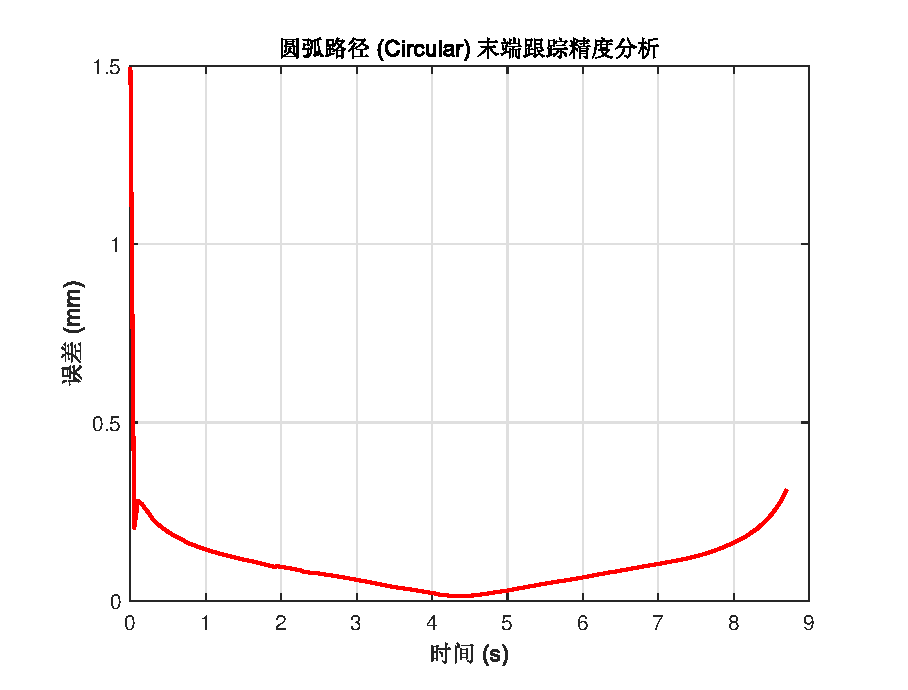
\includegraphics[width = \textwidth]{figures/圆弧精度.eps}
        } % 这里写第二张图的英文描述
             % 第一张子图
            \end{minipage}
    % 中英文总标题
    \caption{末端跟踪精度}
    \label{pic47}
  \end{figure}

\BiSection{本章小结}{Subsubsection}
本章针对水下绳驱机械臂的作业需求，详细开展了笛卡尔空间轨迹规划算法的研究与仿真验证。
首先，建立了直线与空间圆弧的几何离散采样模型，将连续路径转化为离散位姿序列；其次，
设计了带有前序解约束的逆运动学迭代映射算法，有效解决了机械臂在多解空间中的运动连续
性问题。最后，通过 MATLAB 仿真实验对典型工况进行了测试。结果表明，末端跟踪误差保持
在 $10^{-2}$mm 量级，且关节运动平稳、无跳变。仿真结果验证了算法的准确性与鲁棒性，为
后续机械臂在复杂水下环境中的精密作业奠定了坚实的算法基础。





